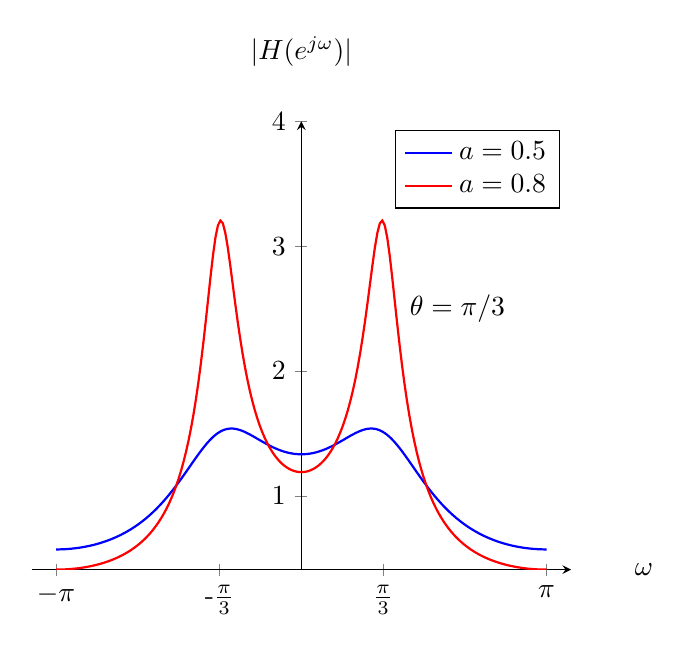
\begin{tikzpicture}
	
	\begin{axis}[
		xlabel=$\omega$,
		ylabel=$|H(e^{j\omega})|$,
		axis lines = middle,
		xmin = -1.1*pi,
		xmax = 1.1*pi,
		ymax = 4,
    	xtick={-3.14159, -1.0472, 1.0472,  3.14159},
    	xticklabels={$-\pi$, -$\frac{\pi}{3}$,  $\frac{\pi}{3}$,  $\pi$},
    	y label style={at={(axis description cs:0.5,1.1)},anchor=south},
    	x label style={at={(axis description cs:1.1,0)},anchor=west},    	
	]
	\def\r{0.5}
	\def\ct{0.5}%cos(theta)
	\addplot[blue, thick, domain=-pi:pi, samples=201] {1/sqrt(1 + 4*\r^2*\ct^2 + \r^4 - 4*\r*\ct*cos(deg(x)) + 2*\r^2*cos(2*deg(x)) -4*\r^3*\ct*cos(deg(x))*cos(2*deg(x)) -4*\r^3*\ct*sin(deg(x))*sin(2*deg(x)) )};
	\def\r{0.8}
	\addplot[red, thick, domain=-pi:pi, samples=201] {1/sqrt(1 + 4*\r^2*\ct^2 + \r^4 - 4*\r*\ct*cos(deg(x)) + 2*\r^2*cos(2*deg(x)) -4*\r^3*\ct*cos(deg(x))*cos(2*deg(x)) -4*\r^3*\ct*sin(deg(x))*sin(2*deg(x)) )};
	\legend{$a=0.5$, $a=0.8$}
	\node at (axis cs:2, 2.5) {$\theta = \pi/3$};
	\end{axis}
\end{tikzpicture}